\documentclass{article}
\usepackage[utf8]{inputenc}
\usepackage{epsfig}
\usepackage{graphicx}
%\usepackage[dvips]{graphics}

	
\title{Tesis. Labrum = Rodete cotiloideo, rodete acetabular, labrum acetabular}
\author{Por Mi}
\date{2017}

	
\begin{document}	
\maketitle	
	\section{Introducción}  
	Descripción general del tema y de cómo se tratará todo. Hacer al final
	
	\section{Análisis descriptivo} 
		\begin{itemize}
			\item Poner de qué se trata, los datos de medicina, las imágenes de medicina, y contexto
			
			Los datos usados en la tesis son datos reales, no se incluyen datos personales de los pacientes, más que su edad, para conservar la privacidad de estos. 
			
			%El problema central es el siguiente: 
			
			%En este proyecto había cuatro radiólogos leyendo imágenes de resonancia magnética de caderas, usando la secuencia estándar (SOC = standard of care) y una nueva llamada IDEAL. Los radiólogos evalúan el daño en el cartílago en la cabeza del fémur usando la "carátula del reloj" para descubrir su localización. A los pacientes con "labral tears" (desgarres) son operados con artroscopía, y el cirujano evalúa el daño "real". La pregunta era si IDEAL era mejor que SOC para visualizar el daño, y evaluar que tan repetibles son las lecturas entre radiólogos y las del mismo radiólogo con las dos secuencias.	
			
			Antes de entrar al análisis, se dará una breve explicación de lo que son las roturas del labrum acetabular, para así comprender mejor los resultados.
			
	        \subsection{Contexto médico}
	        La articulación de la cadera está formada por la cabeza femoral (superficie convexa o bola) y por el acetábulo (cavidad articular). El labrum acetabular es un borde de tejido blando, o fibrocartílago, que rodea el acetábulo. El labrum ayuda a dar estabilidad a la cadera y a proteger la unión entre la cabeza del fémur y el acetábulo. (Fuente: US San Diego Health) 
	        
	        % Imagen de la anatomía de la cadera. Poner fuente
	        \begin{figure}[h!tb]
	        	\centerline{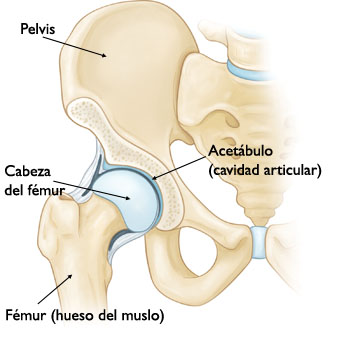
\epsfig{file=cadera,width=3.5cm}}	
	        	\caption{\label{fig:prueba} Anatomía de la cadera.}
	     	\end{figure}
	        
	        El labrum puede sufrir una ruptura debido a lesiones o degeneración.  Este tipo de lesiones son comunes en atletas que practican fútbol, fútbol americano, ballet, gimnasia, hockey y golf, entre otros. (Fuente: MayoClinic)
	        
	        %Imagen de tear. Poner fuente
	        \begin{figure}[h!tb]
	        	\centerline{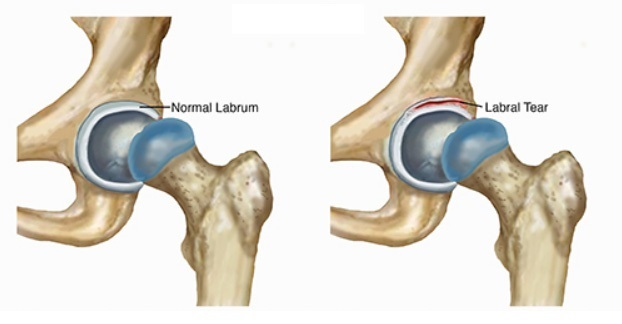
\epsfig{file=tear,width=3.5cm}}	
	        	\caption{\label{fig:prueba} Lesión del labrum acetabular.}
	        \end{figure}
	        
	        Para diagnosticar una lesión se puede hacer uso de radiografías, pero para obtener mayor información se usa la Resonancia Magnética (RM). En caso de que el paciente necesite intervención quirúrgica se recurre a la artroscopía de cadera, que es un procedimiento cuyo objetivo el reinsertar el labrum roto y reparar cualquier anomalía ósea que pueda tener la cadera (Fuente: Clínica Meds). --- La lectura de la RM se hace en términos de horas de un reloj de manecillas, por ejemplo, 12 a 3. ---
	        
			% Imágenes de RM y labrum (reparado). Poner fuente
			\begin{figure}[h!tb]
				\centerline{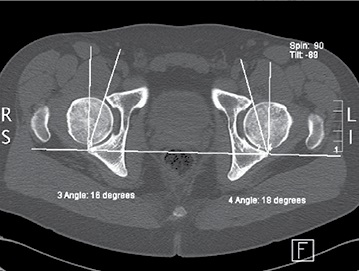
\epsfig{file=mrilabraltear,width=3.5cm}}	
				\caption{\label{fig:prueba} Resonancia magnética de cadera.}
			\end{figure}
			
			\begin{figure}[h!tb]
				\centerline{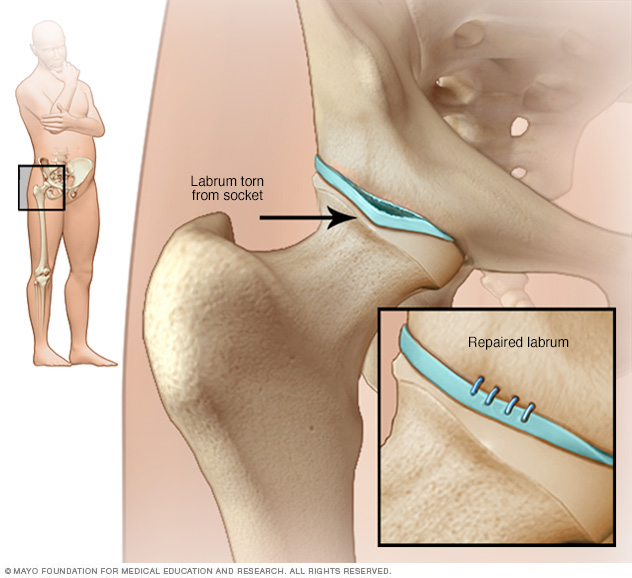
\epsfig{file=labrumreparado,width=3.5cm}}	
				\caption{\label{fig:prueba} Labrum reparado.}
			\end{figure}
				
			
			

			
			\subsection(obtención de los datos)
			\item ¿Cómo obtuve los datos?
			
			Los datos los obtuve
			
			
			
			
			
			
			
			
			
			
			
			
			
			
			
			
			
			
			
			
			
			
			
			
			
			
			
			
			\item ¿Qué datos tiene la base y cómo vienen los datos? en excel, en horas, los pacientes, etc
			\item ¿Cómo se manipularon los datos? ¿Qué se hizo con los NA's? Conversión de reloj a círculo unitario, de horas a radianes ¿Qué se hizo con los que tenían solo una hora (12:00)? ¿Y con los que tenían dos (12:00 a 1, 2:00 a 3)?
			\item Definición de variables Posición y Extensión. Tabla de radianes, rangos, cómo se midieron, etc
			\item Introducir brevemente el análisis descriptivo, i.e., solo decir que mostraré varias gráficas para explicar todo
		\end{itemize}
		
	\section{Análisis gráfico}
	Aquí se va a analizar al EXACTITUD
	Mostrar todas las gráficas y decir qué es lo que se ve en cada una
		
		\begin{itemize}
			\item Posición
				\begin{enumerate}
					\item Gráficas para describir la base: género, lado, edad 
					\item Gráficas en las que comparo los métodos poc cada médico (son 4 por hoja): Ideal vs SOC, Ideal vs Cirujano, SOC vs Cirujano
					\item Gráficas por paciente en la que se comparan los cuatro médicos y cirujanos (son 87 gráficas y por página vienen como 20)
				\end{enumerate}	
			\item Extensión
				\begin{enumerate}
					\item Gráficas para describir la base: género, lado, edad 
					\item Gráficas en las que comparo los métodos poc cada médico (son 4 por hoja): Ideal vs SOC, Ideal vs Cirujano, SOC vs Cirujano
					\item Gráficas por paciente en la que se comparan los cuatro médicos y cirujanos (son 87 gráficas y por página vienen como 20)				
				\end{enumerate}			
		\end{itemize}
	
	\section{Modelos. Aproximación teórica}
	Aquí se va a analizar al PRESICIÓN
	*Checar dónde comencé a usar las deltas
	Poner lo de jtter set.seed, definición del vector de deltas, vector de Métodos (con 0 y 1), y vector de Médicos (con 1, 2, 3 y 4), valores p, pruebas de hipótesis (lo del cociente o ratio -- lo tengo en la libreta el día 26 de julio), ANOVA, modelos
		\begin{itemize}
			\item Modelo1: delta ~ med
			\item Modelo2: delta ~ met
			\item Modelo3: delta ~ med + met
			\item Modelo4: delta ~ med + met + med:met
		\end{itemize}
		
	
	\section{Conclusiones}
	Poner aquí una recapitulación de todo lo que se hizo, y los resultados obtenidos: cúal es el método y médico más acertado, un poco de datos circulares
	
	
	\section{Apéndice}
		\begin{itemize}
			\item Datos circulares: qué son, la función de densidad, porqué no se usaron, limitaciones por los datos, etc (checar correos de Barrios con tesis y la tesis que le mandé al inicio)
			\item Gráfica de pastelitos y una explicación
		\end{itemize}
	
	\section{Bibliografía}
	Fuentes, fotos, etc
	
\end{document}